%=================================================================
\section{Introduction}\label{sec-intro}
\subsection{Problem Statement}
The competation \textit{Google QUEST Q\&A Labeling} is designed to 
improving automated understanding of complex question answer content.
The challenge is to use this new dataset to build predictive algorithms for different subjective aspects of question-answering. 
The question-answer pairs were gathered from nearly 70 different websites, in a "common-sense" fashion.
\begin{figure}[htbp]
    \centering
    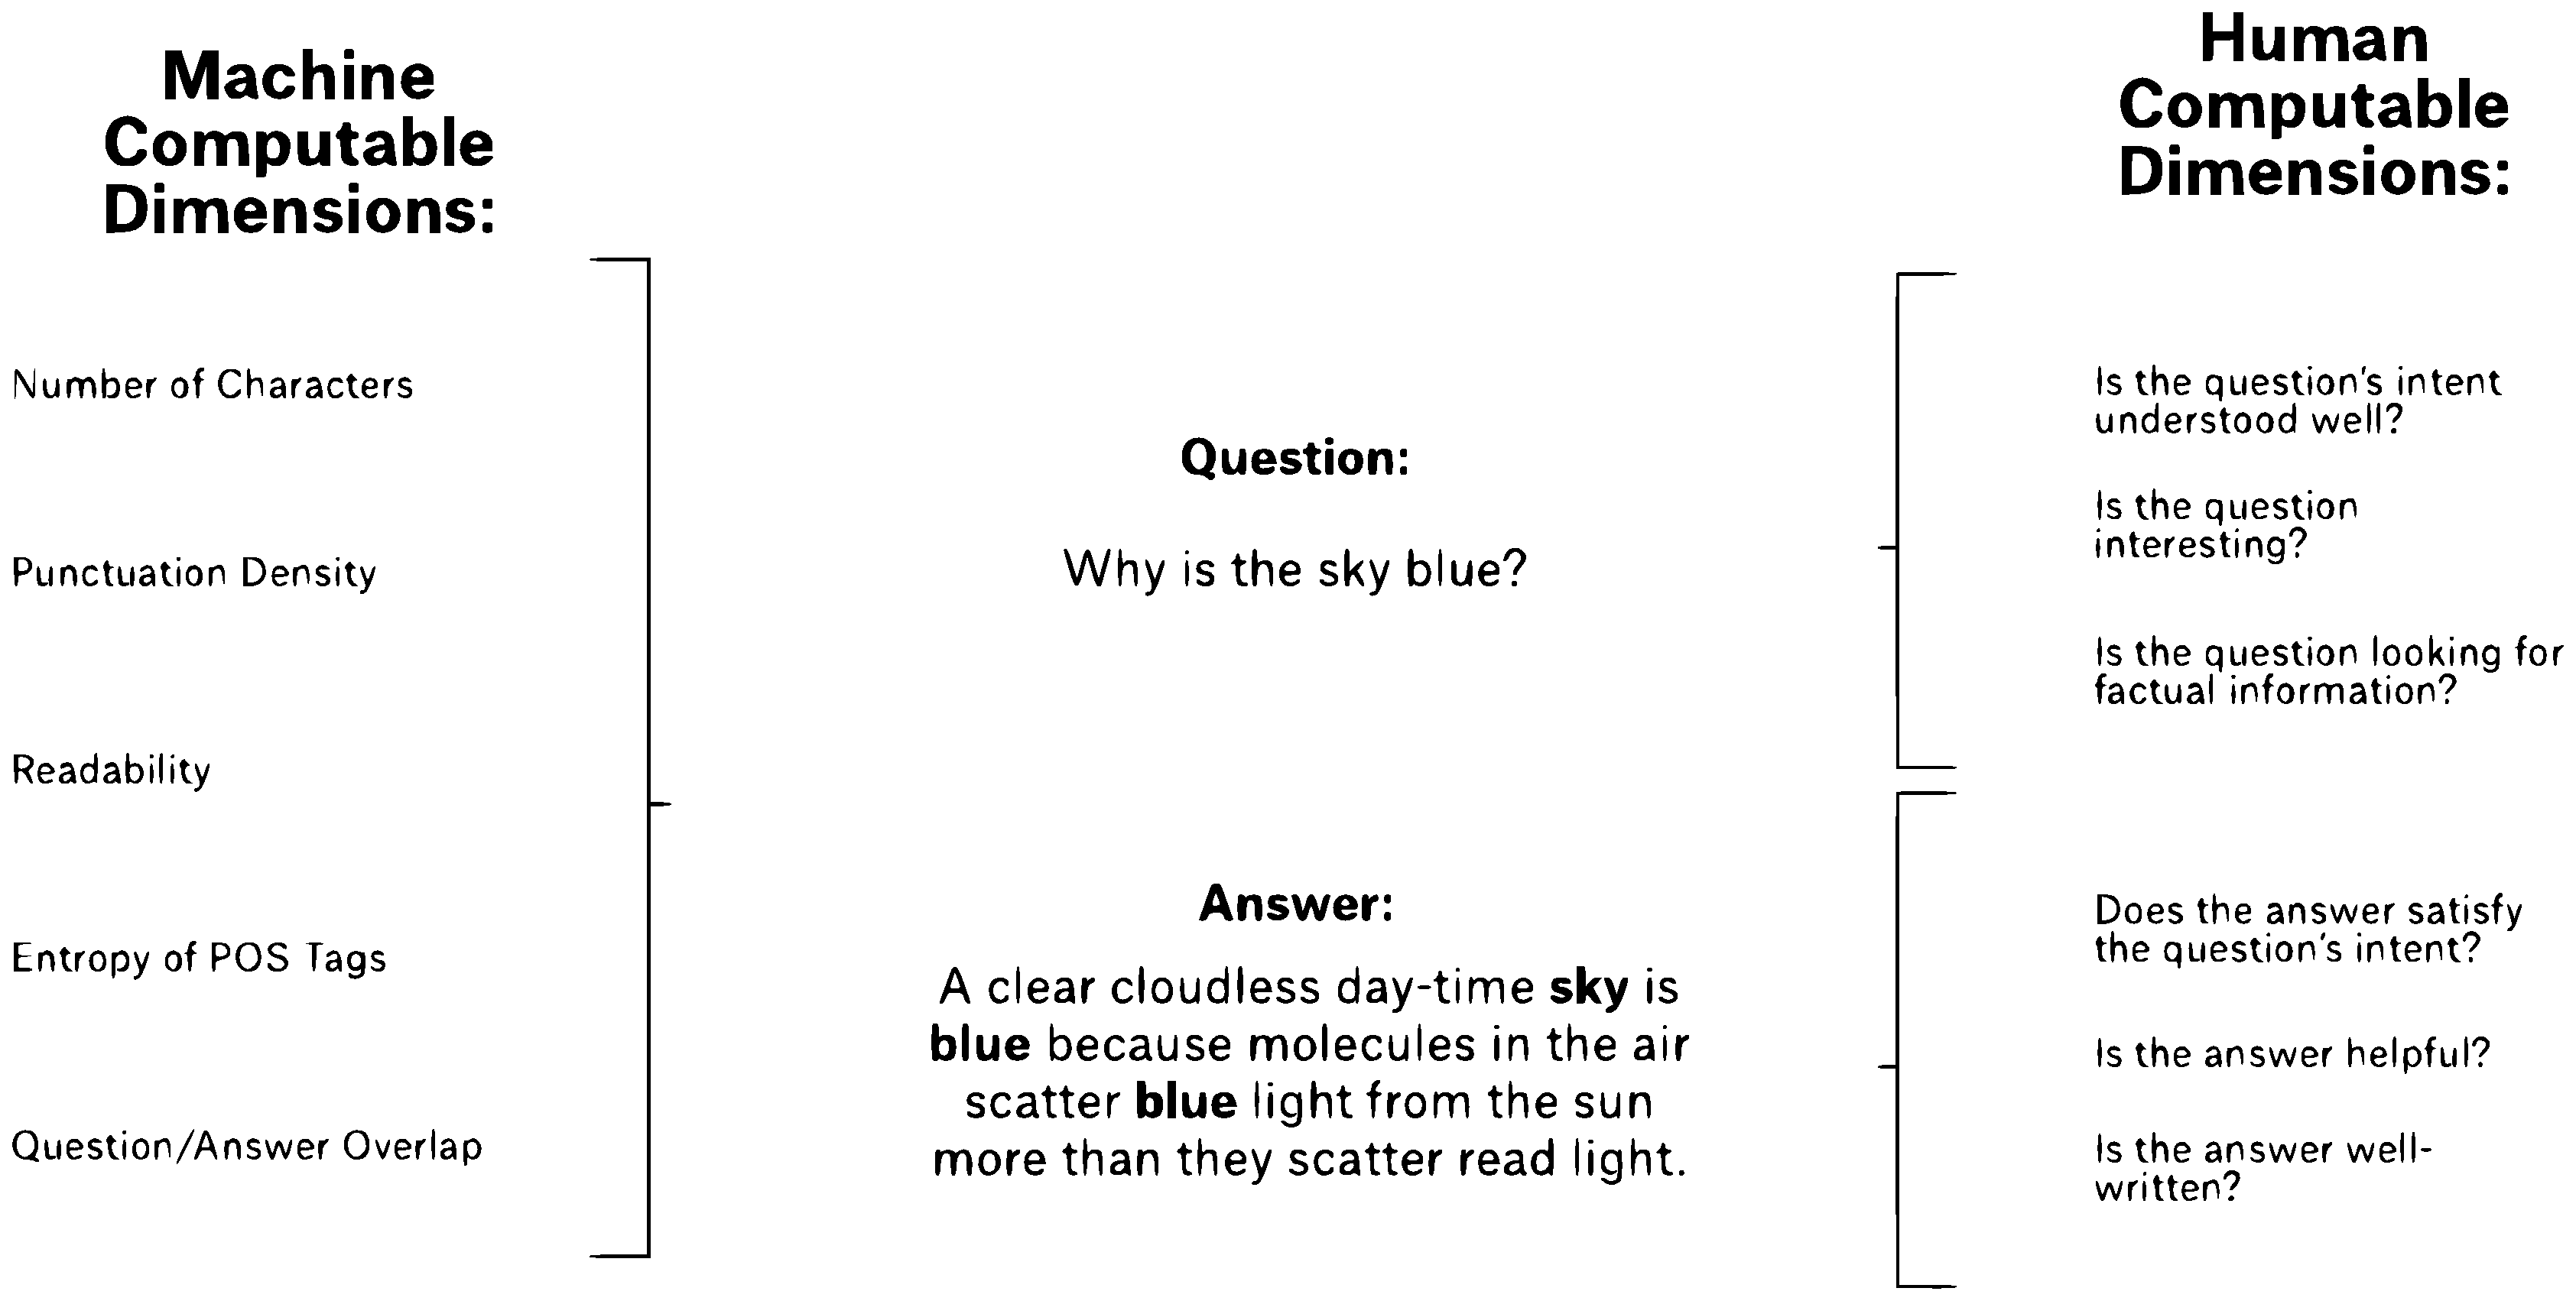
\includegraphics[width=30em]{figures/title.eps}
    \caption{Different between machine and human answer}
    \label{fig:title}
\end{figure}
\subsection{Dataset}
The dataset contains 6049 records in training set and 476 records in test set, with the following features:
\begin{itemize}
    \item Question title\&body
    \item Answer
    \item Host
    \item Category
    \item Question user
    \item Answer user
    \item Url
\end{itemize}
The targets are both continuous values in the range of $[0,1]$, representing the score of this record in the corrsponding dimension.
It contains 21 question related targets and 9 answer related targets.

\subsection{Solution}
Transformer Models such as \textit{Bert} are proven have great performance on many nlp tasks, especially for Question\&Anwser tasks.
In this competation, I will use Bert Model to solve the problem.
\newpage
\section{EDA and Data Preprocessing} \label{sec-eda}
\subsection{Host and Category}
\subsection{Targets}
\subsection{Duplicated Questions}
The competition description has said that:
\begin{itemize}
    \item \emph{The training data contains rows with some duplicated questions (but with different answers). }
    \item \emph{The test data does not contain any duplicated questions.}
\end{itemize}
\begin{table}[htbp]  
    \centering
    \caption{Duplicated Questions}
    \label{tbl:dup_q}
    \begin{tabular}{lc}
        \hline
        Question Title & Count \\
        \hline
        What is the best introductory Bayesian statist...   &12\\
        Important non-technical course for programmers?	    &11\\
        What does mathematics have to do with programm...   &11\\
        How to prevent the "Too awesome to use" syndrome    & 9\\
        How do I deal with a slow and undedicated coll...   & 7\\
        No sound in Ubuntu except at log in	                & 7\\
        What are the benefits of owning a physical book?    & 7\\
        Another instructor is pushing me out of the cl...   & 7\\
        Does "so far, so good" carry a negative connot...   & 6\\
        Good travel games for two players, especially ...   & 6\\
        \dots&-\\
        \hline
    \end{tabular}
\end{table}
\begin{itemize}
    \item The question related targets of these records are not always equle.
    \item It's reasonable to set all question related targets of duplicated questions to its mode or mean.
    \begin{itemize}
        \item \emph{t1:\ question_asker_intent_understanding}
        \item \emph{t2:\ question_body_critical}
        \item \emph{t3:\ question_conversational}
    \end{itemize}
\end{itemize}
    \begin{table}
        \centering
        \caption{The same question-related target of duplicated questions should have the same value in order to reach a better result.}
        \label{tbl:dp_before}
        \begin{minipage}{0.48\linewidth}
        \begin{tabular}{cccc}
            \hline
            qa_id	&t1 &t2 &t3 \\
            \hline
            366	    &1.00000 &1.00000 &0.00000\\
            2536	&1.00000 &1.00000 &0.66667\\
            2591	&1.00000 &1.00000 &1.00000\\
            3349	&1.00000 &1.00000 &1.00000\\
            5543	&1.00000 &1.00000 &0.00000\\
            5989	&1.00000 &1.00000 &1.00000\\
            6041	&0.77778 &1.00000 &0.66667\\
            6215	&1.00000 &0.88889 &0.33333\\
            7003	&0.77777 &1.00000 &1.00000\\
            8328	&1.00000 &1.00000 &0.66667\\
            8867	&1.00000 &1.00000 &0.66667\\
            9137	&1.00000 &1.00000 &0.00000\\
            \hline
        \end{tabular}
    \end{minipage}
    \begin{minipage}{0.48\linewidth}
        \begin{tabular}{cccc}
            \hline
            qa_id	&t1 &t2 &t3 \\
            \hline
            366	    &1.00000	&1.00000	&0.66667\\
            2536	&1.00000	&1.00000	&0.66667\\
            2591	&1.00000	&1.00000	&0.66667\\
            3349	&1.00000	&1.00000	&0.66667\\
            5543	&1.00000	&1.00000	&0.66667\\
            5989	&1.00000	&1.00000	&0.66667\\
            6041	&1.00000	&1.00000	&0.66667\\
            6215	&1.00000	&1.00000	&0.66667\\
            7003	&1.00000	&1.00000	&0.66667\\
            8328	&1.00000	&1.00000	&0.66667\\
            8867	&1.00000	&1.00000	&0.66667\\
            9137	&1.00000	&1.00000	&0.66667\\
            \hline
        \end{tabular}
    \end{minipage}
    \end{table}
\section{Method} \label{sec-method}
\subsection{Embedding}
The idea of vector semantics is thus to represent a word as a point in some multidimensional semantic space.
Vectors for representing words are generally called embeddings, because the word is embedded in a particular vector space.
After convert to embeddings, words with similar meanings are nearby in space.

\subsection{Transformer}
\subsection{Bert}
\section{Experiment and Analysis} \label{sec-experiment}
\subsection{Model Building}
\subsection{Experiment}
\section{Conclusions} \label{sec-conclusions}


The authors would like to thank \ldots

